
\chapter{Evaluation}
\label{cha:789}

The evaluation of the prototype BPMNPA with real-life BPMN diagrams aims to verify the effectiveness of the prototype in generating meaningful BPMN diagram given the correct input parameters.
Specifically, three popular BPMN diagrams has been taken in exam\cite{bpmn2examples}, for every BPMN file a PDDL domain and some PDDL problems have been generated.
In the next sections we will illustrate and discuss how the real-world cases has been modified by the execution of BPMNPA.

\section{Pizza Delivery}
\label{sec:456}
On a modified version of "The Pizza Collaboration" Business Process Diagram we execute BPMNPA. The aim of this test case is to find an alternative path to the standard execution of the BPMN diagram using the set of actions defined in the domain. The diagram generated by BPMNPA represent a viable path to reach the Task "Receive payment" using a newly created set of Tasks and Parallel Gateways.
\begin{center}
\begin{figure}[h!]
		\centerline{\includegraphics[width=1\textwidth]{pizza.eps}}
		\caption{A modified version of the Pizza Collaboration after an alternative path search.}
\end{figure}
\end{center}


\section{Shipment Process}
\label{sec:456}
The next BPMN diagram describes the shipment process of hardware. A process engineer may want to explore the possible ways to optimize this process making its execution faster or cheaper.

With the prototype we obtain a new BPMN diagram inserting a new path for the warehouse worker Lane. This new path aim to reduce the time taken to execute the actions. It has been considered a scenario where in the same warehouse there are multiple packages with the same characteristic, to make the package gathering less expensive. The worker now decides to pick the package within the minor distance between the package location and the pick-area instead of the nearest package to the warehouse worker, diminishing the walk time.
\begin{center}
\begin{figure}[h!]
		\centerline{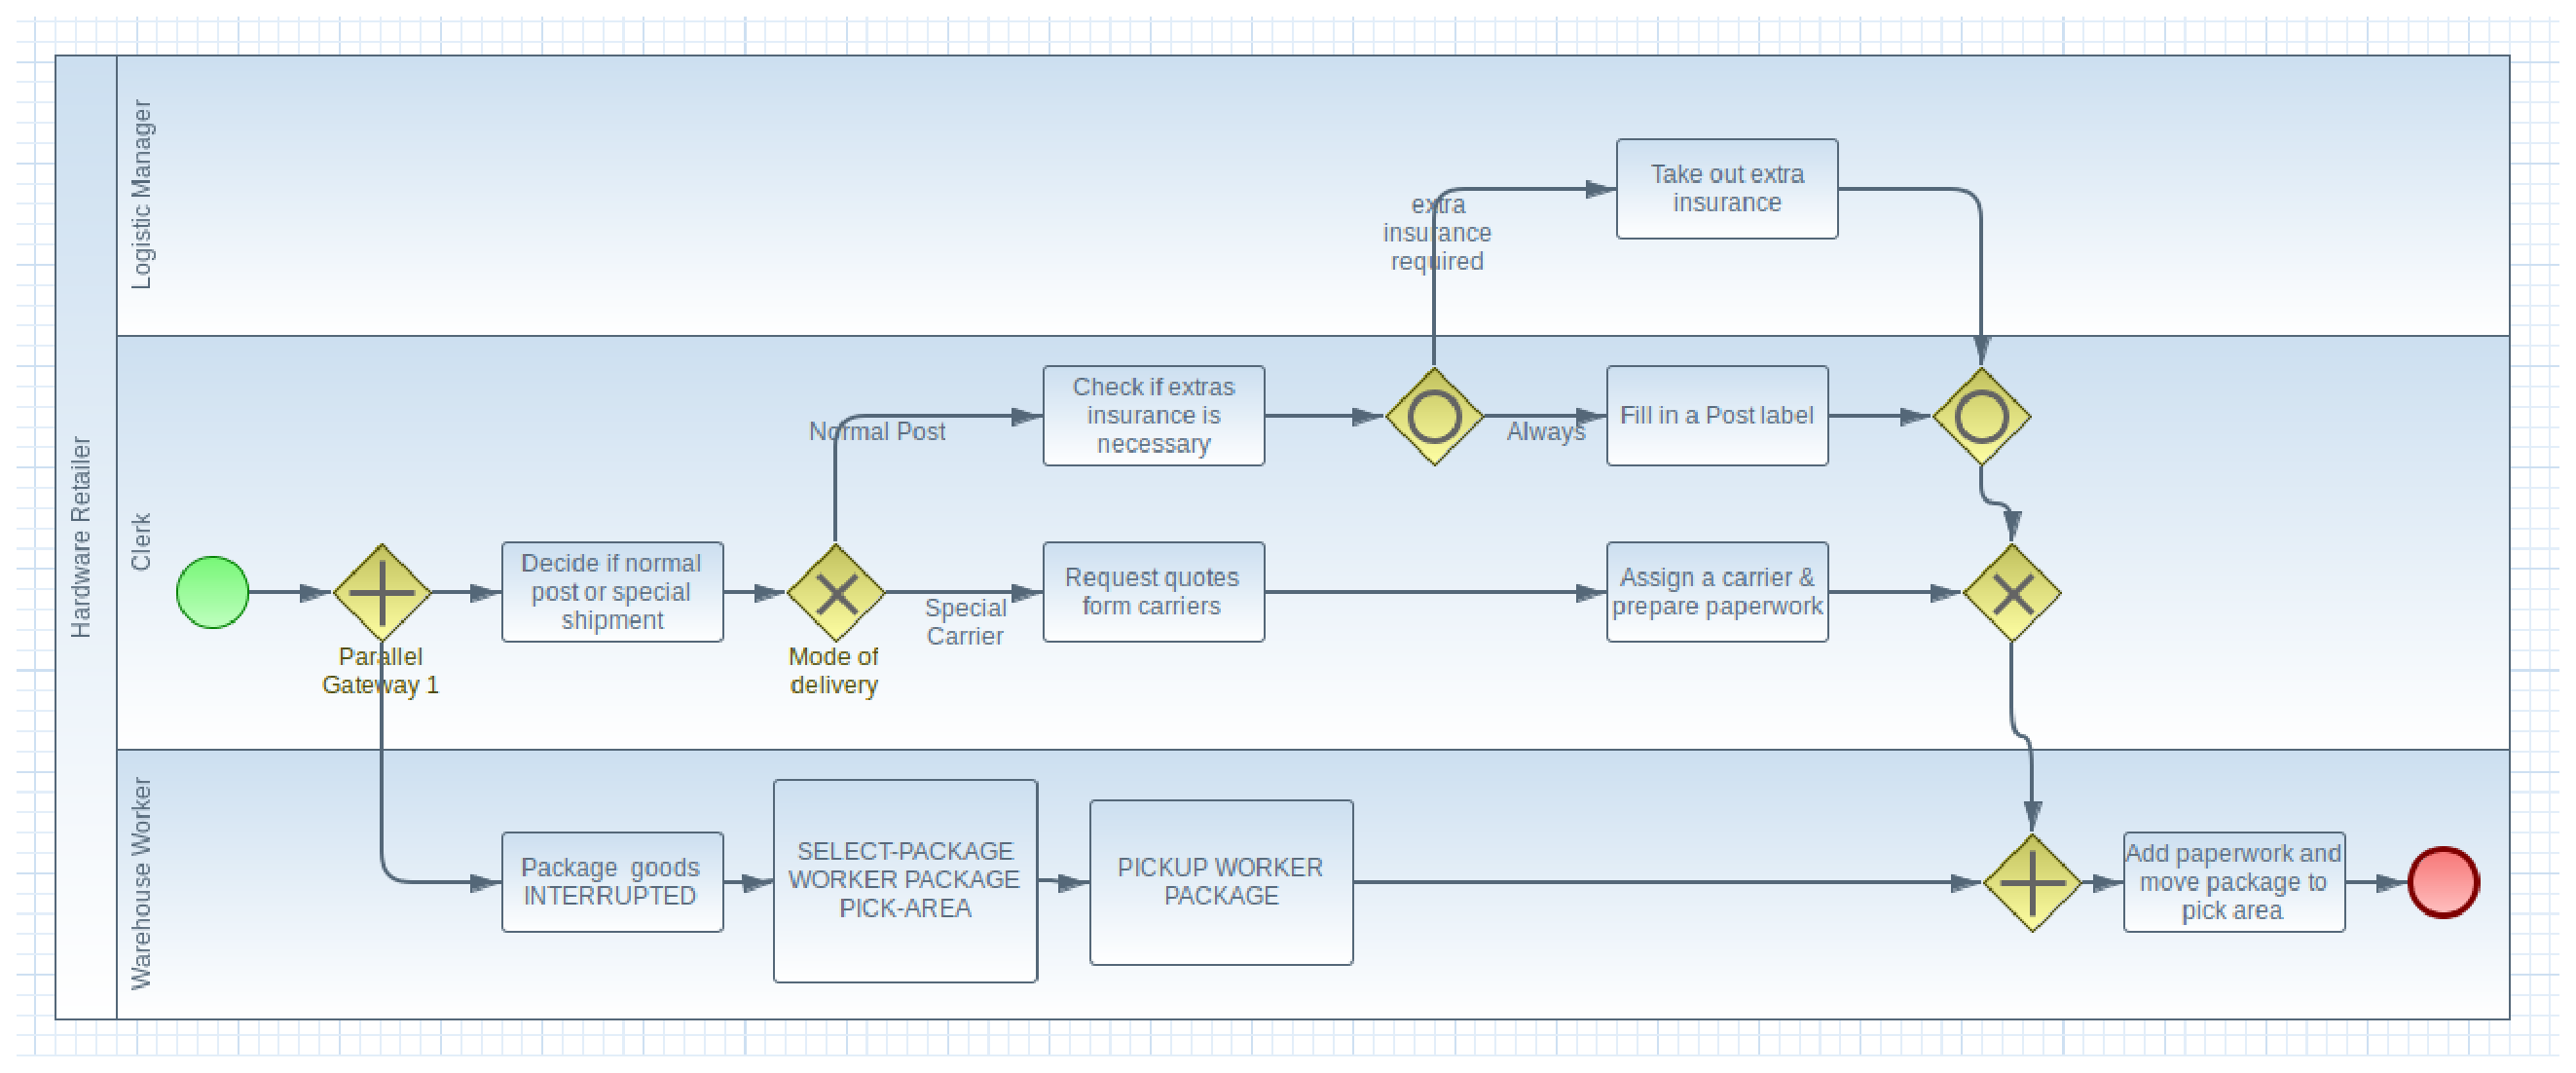
\includegraphics[width=0.8\textwidth]{warehouse.eps}}
		\caption{The Shipment Process optimized to reduce walk-time.}
\end{figure}
\end{center}

\section{Nobel Prize Example}
\label{sec:456}
In this case we considered a run-time error during the execution of the task "Discuss Nominations (meeting 1)" in the Noble Assembly Lane. We have considered the task to have as precondition the successful completion of "Submit Report with Recommendations" and as post-conditions the end of the meeting.


We consider that the run-time error, in this case, has been thrown by the fact that the meeting can start only if at-least four people are present. BPMNPA has created a new set of elements in order to exit this error state and restore the execution, by using available agents, to fulfill the goals of the Task "Discussion Nominations (meeting 1)" and to make feasible the execution of "Discussion Nominations (meeting 2)".

\begin{center}
\begin{figure}[h!]
		\centerline{\includegraphics[width=1\textwidth]{noble.eps}}
		\caption{The result of recovering a run-time error in the Nobel Prize example.}
\end{figure}
\end{center}
